\chapter[Desenvolvimento da Proposta]{Desenvolvimento da Proposta}

Este capítulo apresenta o uso de metodologias e conceitos relacionados à Engenharia de Software que serão aplicados no desenvolvimento da proposta descrita no capítulo anterior.

A metodologia a ser utilizada é híbrida: contém elementos de metodologias clássicas e conhecidas na área de Engenharia de Software. Para melhor visualização da metodologia, um processo de execução de atividades foi modelado e está detalhado neste capítulo.

A seção 4.1 deste capítulo apresenta uma contextualização da proposta. A metodologia de execução da proposta, seção 4.2, apresenta a modelagem do processo de desenvolvimento de software adotado para a execução deste projeto de TCC, com detalhes sobre as atividades contidas em cada uma das fases e seus respectivos objetivos. Os cronogramas para as duas partes de execução do TCC são apresentados e detalhados na seção 4.3.

\section{Introdução}
O projeto de Engenharia de Software a ser desenvolvido como parte do trabalho de conclusão de curso consiste em uma arquitetura para uma plataforma virtual onde as funcionalidades serão tratadas como serviços no contexto arquitetural. Os serviços ou funcionalidades desta plataforma virtual consistem de aplicações de \textit{software} desenvolvidas no contexto do grupo de orientação do Professor Doutor Sérgio Antônio Andrade de Freitas e trabalhos desenvolvidos no Laboratório Fábrica de Software da Universidade de Brasília. A plataforma virtual é um meio de disponibilizar tais trabalhos para uso pela comunidade.

A proposta descrita no capítulo 3 será desenvolvida utilizando-se de alguns conceitos de metodologias de desenvolvimento e de gerenciamento de projetos de software, adaptadas conforme as necessidades deste projeto.

\section{Metodologia de Execução da Proposta}
Um projeto de Engenharia de Software deve ser realizado utilizando-se de metodologias, técnicas e ferramentas disponíveis relacionadas à esta área de conhecimento, sendo sempre adaptadas de acordo com o projeto a ser desenvolvido visando, assim, o sucesso na conclusão do projeto.

Entre as diversas metodologias de desenvolvimento de software existentes, foi decidido pela adoção de uma metodologia híbrida para o desenvolvimento deste projeto. Esta metodologia híbrida contém alguns conceitos relacionados ao RUP (Rational Unified Process) e outros relacionados à metodologia ágil de desenvolvimento, mais especificamente o Scrum. 

A metodologia híbrida adotada é composta pelas fases do RUP e alguns de seus artefatos. Envolve também o conceito de histórias de usuário, que em sua maioria serão tratadas como histórias técnicas  neste projeto. Além disso, o modelo de desenvolvimento é iterativo e incremental, tornando a identificação de falhas e correção das mesmas mais eficiente, assim como a identificação de novas necessidades para que a arquitetura e o protocolo de comunicação propostos sejam implementados.

Foi modelado um processo para a execução das atividades necessárias para a realização do trabalho de conclusão de curso, tanto para que a proposta pudesse ser elaborada, quanto para o planejamento e execução desta. A figura \ref{processo_tcc} ilustra o processo, ainda em andamento, e contém os aspectos relacionados à metodologia adotada.

\begin{figure}[htb]
\centering
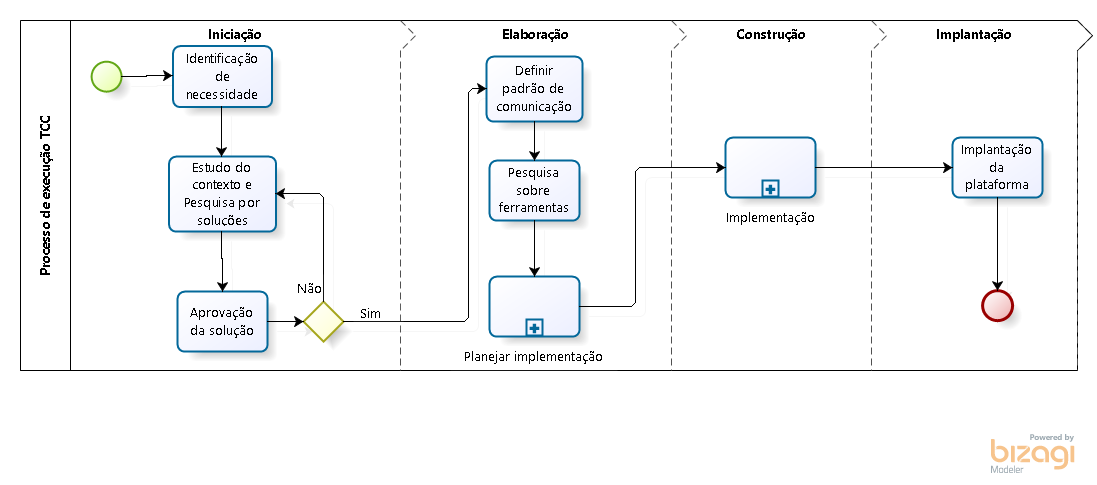
\includegraphics[width=1\textwidth]{figuras/processo_tcc.PNG}
\caption{Processo de elaboração e execução do TCC.}
\label{processo_tcc}
\end{figure}

A figura \ref{processo_tcc} apresenta o processo em execução, com suas fases e as atividades correspondentes de  cada fase. O processo foi dividido de acordo com as fases do RUP: iniciação, elaboração, construção e implantação. A fase de iniciação contém as atividades de \textit{Identificação de necessidade}, \textit{Estudo do contexto e Pesquisa por soluções} e \textit{Aprovação da Solução}: uma vez que a necessidade foi identificada, foi realizado um estudo sobre o contexto e uma pesquisa por soluções arquiteturais adequadas.

A fase de elaboração contém atividades que procuram refinar conceitos relacionados ao este modelo arquiteural escolhido e definir padrões e ferramentas que serão utilizadas na fase de construção, além de obter um plano de execução para a fase seguinte. Assim, foram realizadas as atividades de definição de um padrão de comunicação para a arquitetura, uma pesquisa sobre ferramentas que podem ser úteis no desenvolvimento da arquitetura da plataforma virtual e o planejamento da fase de construção.

Na fase de construção o planejamento realizado será executado. É nesta fase em que adaptações deverão ser feitas, tanto na plataforma virtual quanto em aplicações que fornecerão serviços. A fase de construção é constituída de ciclos iterativos e incrementais e será detalhada mais adiante.

A última fase definida no processo é a fase de implantação. Nesta fase a plataforma deverá ser implantada e homologada para uso pela comunidade.

Ao final do TCC 1, as fases do processo executadas foram a iniciação e a elaboração do projeto. O processo definido poderá ser readaptado durante as próximas etapas de realização do trabalho. Os processos definidos para as fases de construção e implantação podem ser repetidos sempre que uma nova funcionalidade implementada por um serviço seja incorporada à plataforma virtual criada.

\subsection{Planejamento da Implementação}
Durante a fase de construção, um subprocesso definido foi o de planejamento da implementação (subprocesso da fase de construção do projeto). As atividades e o fluxograma deste subprocesso podem ser visualizados na figura \ref{subprocesso_planejamento}.

\begin{figure}[htb]
\centering
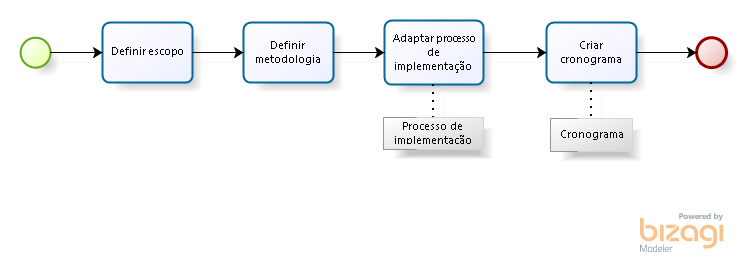
\includegraphics[width=1\textwidth]{figuras/subprocesso_planejamento.PNG}
\caption{Fluxograma e atividades do subprocesso Planejar Implementação.}
\label{subprocesso_planejamento}
\end{figure}

A figura \ref{subprocesso_planejamento} exibe as atividades realizadas durante a fase de elaboração definida no processo e que já foi realizada durante o TCC 1. As atividades são \textit{Definir escopo}, \textit{Definir metodologia}, \textit{Adaptar processo de implementação} e \textit{Criar cronograma}. No início do planejamento o escopo do que será entregue ao final do trabalho de conclusão de curso foi definido. Esta atividade foi seguida da definição de uma metodologia de desenvolvimento de software para a execução do projeto e, baseando-se na metodologia definida, um processo a ser seguido para a implementação da arquitetura foi adaptado. Por fim, um cronograma de execução da implementação foi criado.

Na atividade de definição do escopo não foi definida a aplicação que será adaptada e incorporada à plataforma como um serviço a fim de demonstrar a proposta feita. Esta escolha deverá ser feita durante na fase de construção.

A metodologia definida foi do tipo híbrida, que utiliza conceitos das metodologias tradicional (RUP) e ágil (Scrum).

\subsection{Fase de Construção}
O uso de uma arquitetura baseada no modelo SOA não elimina o trabalho necessário para a inserção de novos serviços: o seu uso visa minimizar os reparos que devem ser feitos para que uma nova funcionalidade seja incorporada ao sistema, promovendo extensibilidade e flexibilidade à arquitetura construída.

A fase de construção do processo definido tem como objetivo a implementação da plataforma virtual de acordo com os requisitos básicos levantados e que foram importantes para a proposta da solução e a adaptação de uma aplicação existente para ser incorporada à plataforma. Em um contexto onde novos serviços serão inseridos na plataforma em um tempo posterior à execução do TCC, esta fase será também executada (figura \ref{subprocesso_implementacao}).

\begin{figure}[htb]
\centering
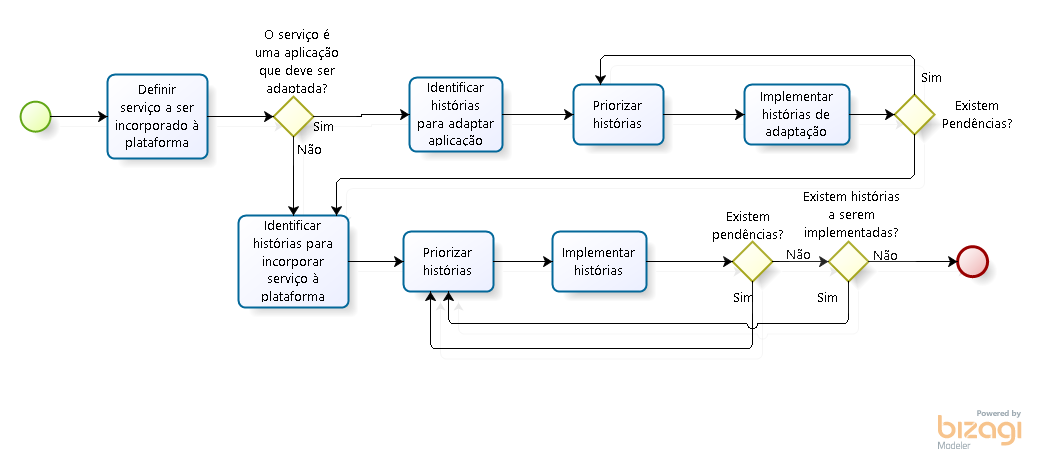
\includegraphics[width=1\textwidth]{figuras/subprocesso_implementacao.PNG}
\caption{Fluxograma e atividades da fase de construção.}
\label{subprocesso_implementacao}
\end{figure}

A figura \ref{subprocesso_implementacao} exibe o fluxograma de atividades a serem executadas no subprocesso de implementação definido na fase de construção da plataforma virtual. As atividades a serem realizadas são dependentes da definição do serviço que será incorporado à plataforma, pois, caso um novo serviço seja uma aplicação que deve ser adaptada, as atividades referentes à adaptação desta deverão ser executadas. Se o novo serviço ou funcionalidade, não for uma aplicação a ser adaptada para fornecer suas operações, pode-se executar as atividades e tarefas referentes à construção da plataforma (no caso do trabalho de conclusão de curso) ou adaptação desta para que a nova funcionalidade seja disponibilizada na plataforma.

Um dos conceitos ágeis utilizados no subprocesso de implementação é o de histórias de usuário: descrição de funcionalidades que agregam valor ao produto final a ser entregue, escrita de maneira simples e facilmente entendida. As histórias a serem elicitadas consistirão tanto de histórias que descrevem funcionalidades, quando de histórias técnicas, que tratam de adaptação e implantação de tecnologias e outros aspectos mais relacionados à parte técnica do desenvolvimento de software do que à funcionalidades.

Outro conceito associado à metodologia ágil de desenvolvimento de software é o de \textit{sprints}. Por se tratar de um modelo criado para ser iterativo e incremental, a fase de construção definida para este TCC consistirá de \textit{sprints} com períodos definidos de 1 (uma) semana. Foi estabelecido que a quantidade de \textit{sprints} será de 8 a 10.

Durante a fase de construção em que as atividades de adaptação de uma aplicação existente e de implementação da plataforma virtual (com o auxílio do ESB selecionado) serão executadas. Estas atividades serão executadas de forma interativa e incremental. Desta forma, serão realizados testes para verificar a corretude e completude da integração entre as aplicações. Na modelagem do processo os testes se encontram implícitos, pois à medida em que partes das adaptações e implementações estiverem prontas, testes para validar e verificar a comunicação serão executados.

O método adotado para teste consistirá em passos sistemáticos que simulem a troca de dados entre aplicações utilizando-se o ESB. O mecanismo de registro de \textit{log} de operações também será útil para os testes a serem realizados, pois exibem os processamentos executados pelo ESB.

Quando finalizadas a adaptação da aplicação e a implementação da plataforma virtual, a fase de implantação será executada. Nesta última fase testes de homologação do resultado final deste projeto serão realizados. Esta fase estará finalizada quando os testes de homologação forem realizados.

As fases de construção e de implantação serão executadas durante a realização do TCC2.

\section{Cronograma de Execução do TCC}
Para o desenvolvimento da proposta e completude da mesma com sucesso foi criado um cronograma para as fases de construção da proposta aqui feita e de implantação do produto final obtido. O cronograma contém as atividades a serem realizadas, bem como os prazos relacionados a cada uma das atividades e pode ser visualizado na tabela \ref{cronograma_tcc2}.

\begin{table}[!h]
\centering
\caption{Cronograma de atividades relacionadas ao TCC 2}
\label{cronograma_tcc2}
\begin{tabular}{|p{9cm}|c|c|c|c|c|}
\hline
Atividade                                                   & \multicolumn{1}{l|}{Jul} & \multicolumn{1}{l|}{Ago} & \multicolumn{1}{l|}{Set} & \multicolumn{1}{l|}{Out} & \multicolumn{1}{l|}{Nov} \\ \hline
Análise de ferramentas a serem utilizadas                   & X                           &                             &                              &                            &                             \\ \hline
Implantação da ferramenta escolhida                         & X                           &                             &                              &                            &                             \\ \hline
Adaptação de uma aplicação já desenvolvida e Testes         &                             & X                              & X                            & X                          &                              \\ \hline
Implementação da plataforma virtual e Testes                &                             & X                          & X                            & X                          &                             \\ \hline
Implantação da plataforma virtual                           &                             &                            & X                          & X                            &                             \\ \hline
Escrita do TCC 2                                            &                             &                             &                            & X                            & X                           \\ \hline
\end{tabular}
\end{table}


\begin{itemize}
\item \textbf{Análise de ferramentas a serem utilizadas:} será selecionada uma ferramenta que fornece os serviços de roteamento, adaptação de tecnologias e tratamento de formatos de dados e de mensagens. Para que isso ocorra, algumas das ferramentas levantadas serão analizadas com mais rigor para que uma seja eleita. A análise consistirá de testes de implantação da ferramentas, bem como de uma avaliação das funcionalidades e da facilidade de uso e aprendizagem.
\item \textbf{Implantação da ferramenta escolhida:} após a escolha da ferramenta, esta deverá ser implantada em um servidor que tenha capacidade para tal. A implantação deverá facilitar o uso da ferramenta durante as atividades posteriores.
\item \textbf{Adaptação de uma aplicação já desenvolvida e Testes:} aplicações já desenvolvidas podem não estar preparadas para serem incorporadas à plataforma virtual como um serviço. Para que isto ocorra, será selecionada uma aplicação para ser adaptada, sendo assim possível de ser disponibilizada na plataforma. Esta atividade também consiste em fazer com que as operações do novo serviço sejam acessadas via o protocolo estabelecido. Testes serão realizados para assegurar que o comportamento esperado da aplicação seja o mesmo ao final da adaptação da aplicação existente.
\item \textbf{Implementação da plataforma virtual e Testes:} nesta atividade, a plataforma virtual será criada e o serviço que foi adaptado deverá ser incorporado a tal plataforma. Aqui serão implementados o uso do protocolo de comunicação estabelecido, bem como o uso da ferramenta ESB escolhida. Para assegurar a corretude e completude do escopo definido, serão realizados testes sistemáticos. Estes testes serão executados por meio da troca de mensagens entre aplicações utilizando o ESB escolhido.
\end{itemize}

As atividades de adaptação de uma aplicação e a incorporação desta aplicação como um serviço à plataforma virtual serão realizadas de maneira iterativa e incremental. Isto justifica o uso de um método de desenvolvimento de software capaz de fornecer suporte para que iterações sejam executadas. A intenção é ter pelo menos uma aplicação adaptada ao padrão do protocolo estabelecido e sendo utilizada na arquitetura como um serviço.

Com relação às atividades realizadas durante o desenvolvimento do TCC 1, a tabela \ref{cronograma_tcc1} contém seus registros e os seus respectivos períodos de execução.


\begin{table}[!h]
\centering
\caption{Cronograma de atividades relacionadas ao TCC 1}
\label{cronograma_tcc1}
\begin{tabular}{|p{9cm}|c|c|c|c|c|c|}
\hline
Atividade                                                   & \multicolumn{1}{l|}{Jan} & \multicolumn{1}{l|}{Fev} & \multicolumn{1}{l|}{Mar} & \multicolumn{1}{l|}{Abr} & \multicolumn{1}{l|}{Mai} & \multicolumn{1}{l|}{Jun} \\ \hline
Identificação da necessidade                                & X                           &                             &                              &                            &                             &                              \\ \hline
Leituras sobre modelos arquiteturais                        & X                           &                             &                              &                            &                             &                              \\ \hline
Pesquisa sobre o modelo arquitetural mais adequado          & X                           & X                             &                              &                            &                             &                              \\ \hline
Pesquisa sobre trabalhos relacionados                       & X                           & X                        &                              &                            &                             &                              \\ \hline
Levantamento inicial de ferramentas ESB                    &                             & X                        & X                            &                            &                             &                              \\ \hline
Definição do padrão de comunicação utilizado                &                             &                          & X                            &                            &                             &                              \\ \hline
Escrita do TCC 1                                            &                             &                             &                              & X                           & X                           & X          \\ \hline
\end{tabular}
\end{table}
